\documentclass{article}
\usepackage[utf8]{inputenc}
\usepackage{caption}
\usepackage[margin=1in]{geometry}
\usepackage{graphicx}
\usepackage{pdfpages}
\usepackage{float}
\pdfminorversion=7

\begin{document}
\begin{titlepage}


\centering
\vspace*{2cm}
{\Huge Final Project Report\par}
\vspace{.25cm}
{\LARGE Course Evaluation System\par}
\vspace{1cm}
{\Large Team EVAL\par}
\vspace{.2cm}
{\Large Jovon Craig, Sam Elliott, Yuanqi Guo, Robert Judkins, and Stanley Small\par}
\vspace{1cm}
{\Large Client: Dr. Harlan Onsrud\par}
\vspace{1cm}
{\Large May 7, 2019\par}
\vspace{11cm}

University of Maine - Spring of 2019 - COS 497

Instructor: Professor Terry Yoo

\end{titlepage}

\newpage

\begin{center}
{\includegraphics[scale=.2]{images/team_logo.png}} \\ 	\bigskip
{\LARGE Course Evaluation System } \\ \medskip
{\large Final Project Report } \\ \medskip
\end{center}

\tableofcontents

\newpage

\section{Introduction}

\subsection{Purpose of This Project}

For our capstone project, Team EVAL is creating a Course Evaluation System, a web application designed to be intuitive and versatile for college instructors. This new system, which will be tested first at the University of Maine, allows one to quickly create course evaluation surveys and review their responses. Our goal is to have a fully working evaluation system for use at the end of the Spring 2019 semester. By making and documenting the software, the team will have gained valuable skills in software engineering, programming, and technical writing.

\subsection{Purpose of This Document}

This final project document gives an overview of our course evaluation system, the purpose of it, and why we believe it is useful. We first talk about existing evaluation creation software and how they are not tailored to college instructors and administrators, unlike our system. The next section goes into more detail about the system, discussing its requirements, user interface, and architecture. The last section describes what we will deliver to the client, our progress on creating the system so far and the steps we still need to take to successfully complete the project.

This document is intended for the development team, the product client, and potential users of the system. Team EVAL needs this document to guide the products development. The client, Professor Harlan Onsrud, also needs it to verify that we are designing the system according to his needs. The document helps the software's users by informing them what the system is designed to do and how it specifically helps them with their work.

\subsection{References}

Craig, J., Elliott, S., Judkins, R., \& Small, S. 29 October 2018. \textit{System Requirements Specification.}
\vspace{3mm}\newline
Craig, J., Elliott, S., Judkins, R., \& Small, S. 16 November 2018. \textit{System Design Document.}
\vspace{3mm}\newline
Craig, J., Elliott, S., Judkins, R., \& Small, S. 30 November 2018. \textit{User Interface Design Document.}
\vspace{3mm}\newline
Craig, J., Elliott, S., Guo, Y., Judkins, R., \& Small, S. 14 March 2019. \textit{Code Inspection Report.}
\vspace{3mm}\newline
Craig, J., Elliott, S., Guo, Y., Judkins, R., \& Small, S. 4 April 2019. \textit{Administrator Manual.}
\vspace{3mm}\newline
Craig, J., Elliott, S., Guo, Y., Judkins, R., \& Small, S. 18 April 2019. \textit{User Manual.}
\vspace{3mm}\newline
Onsrud, H. ``Example Question Selection Form.'' See Appendix H.
\vspace{3mm}\newline
Onsrud, H. ``Example Results Display.'' See Appendix I.
\vspace{3mm}\newline
LimeSurvey: The online survey tool - open source surveys. (n.d.). Retrieved from

https://www.limesurvey.org/.

\section{Purpose of This System}

\subsection{Our Problem}

In 2015, there were more than 4,600 higher-education institutions in the United States. Virtually all of them offer a breadth of college courses for students to complete and take them through their academic careers. At the end of a course, students typically fill out an evaluation so that teachers know what they are doing right and wrong. Unfortunately, many institutions, such as the University of Maine, are behind in using technology for this task.

The University of Maine has traditionally used Scantron sheets for course evaluation forms. As Team EVAL knows, filling in tiny bubbles with pencil and paper is tedious. It is also hard work for the college administration to use Scantron sheets. They need to scan the forms for every student in every course, and the data then needs to be collected in a form that is readable for instructors. The University of Maine must upgrade to keep with the times and exploit today's technology.

\subsection{Existing Survey Software}

Several software solutions currently exist that allow users to create, modify, and publish surveys. One notable example is LimeSurvey, a free and open-source tool that is operated online. The team acknowledges the immense amount of work put into creating LimeSurvey, with its selection of question types, scalability, visualization features, and other powerful functionality. However, LimeSurvey has always been general-purpose software; it is aimed at multiple types of users who want to make surveys.

College teachers and administrators need to jump through hoops to use a tool like LimeSurvey which are not always easy or intuitive. Their evaluations are highly standardized and they are sent to potentially hundreds of students. LimeSurvey and similar software do not account for these qualities. A college instructor would have to manually input every field, question, and class roll into each evaluation from scratch.  UMaine is using another service, Blue by Explorance, that has the necessary functionality, but it is expensive to use for a university and impossible to use for individuals. These are some of the reasons why our client, Dr. Onsrud, wants us to create an evaluation system better suited to instructors.

\newpage

\section{About This System}

\subsection{System Requirements}

Near the beginning of the project, we met with Professor Onsrud to solicit the system requirements, what the evaluation system must do to function as Dr. Onsrud intends. The System Requirements Specification (SRS) divides the requirements into two categories. The functional requirements specify the major actions a user can perform with the system. They are listed in Table 1 below:

\begin{center}

\begin{tabular}{|p{1.5cm}|p{1.5cm}|p{3.5cm}|p{6cm}|} 
\hline
\textbf{Number} & \textbf{Priority} & \textbf{Name} & \textbf{Description} \\
\hline
1 & 5 & Log in to system & A user logs in with a Google e-mail address and password \\ 
\hline
2 & 5 & Create evaluation & A user creates a new evaluation form for a class \\ 
\hline
3 & 5 & Edit evaluation & A user enters and edits information and questions for an evaluation form \\  
\hline
4 & 5 & Publish evaluation & A user publishes an evaluation form \\
\hline
5 & 5 & View evaluation results & The user reviews a course's or category of courses' results \\ 
\hline
\end{tabular}
\captionof{table}{Functional requirements}
\end{center}

The non-functional requirements state the system's qualities that are irrelevant to how the program behaves. They are listed below in Table 2:

\begin{center}
\begin{tabular}{|p{1.5cm}|p{1.5cm}|p{8cm}|}
\hline
\textbf{Number} & \textbf{Priority} & \textbf{Description} \\
\hline
1 & 3 & The software should be supported by the latest versions of Windows, Mac, Linux, iOS, and Android.\\ 
\hline
2 & 4 & The software should be accessible by the latest versions of Safari, Chrome, Firefox, and Edge.\\ 
\hline
3 & 5 & All questions entered by the teacher or administrator shall appear on the output survey.\\  
\hline
4 & 5 & All data stored in the program's database shall be valid.\\
\hline
5 & 5 & All collected survey data shall not be alterable.\\ 
\hline
6 & 4 & Teachers shall not be able to access data of courses other than their own.\\ 
\hline
7 & 3 & The mean time between failures should be at least 60 minutes.\\ 
\hline
8 & 5 & Students shall have no access to any data stored by the program.\\ 
\hline
9 & 5 & All survey responses (except signed \newline comments) shall be anonymous.\\ 
\hline
10 & 2 & The software should scale to at least three universites, 1000 courses per semester, 1000 teachers per university, and 500 students per course.\\  
\hline
11 & 1 & The software should not exceed 500 MB in size.\\
\hline
12 & 4 & The software's source code shall be open-source and shall use a GPLv2 license.\\ 
\hline
13 & 4 & The licensing requirements of any non-original code shall be met.\\ 
\hline
14 & 4 & The software shall meet UMaine AFUM requirements.\\ 
\hline
\end{tabular}
\captionof{table}{Non-functional requirements}
\end{center}

\subsection{System Architecture}

\begin{center}
\begin{figure}[H]
\centering
\vspace{2mm}
{\includegraphics[scale=.75]{images/component_diagram.png}}
\captionof{figure}{Component diagram of the system}
\end{figure}
\end{center}

Our system features a modular design, with many distinct parts which communicate via an API. The front end implements the user interface, written in JavaScript. The back end communicates with the system's databases and is written in Python. We are using two databases, one maintained by LimeSurvey and another maintained by our system. Additionally, the API will communicate with Google Authentication to authenticate users. The design and implementation of our system can be found in the System Design Document (SDD). The system's components are displayed in Figure 1 above.

By maintaining a modular approach to the design of the system, team members can work independently on individual parts, which will then undergo integration testing. Moreover, by keeping the LimeSurvey codebase separate from our system, we can update LimeSurvey without disrupting other parts of the code.

\subsection{Our Process}

When developing our product, we used the scrum framework. Our process subscribes to both process-driven and agile methodologies. Completion of the project requires a strict timeline which corresponds with the academic year, better managed as a process. However, our team regularly collaborates with the client to ensure the correct product is built. Our team follows a spiral methodology with each
iteration producing a working prototype. We use Github to store and maintain the code, along with Docker to ensure our code runs in a familiar environment on different machines. Our class meets twice a week and we have weekly standup meetings.

\begin{center}
\begin{figure}[H]
\centering
\vspace{2mm}
INSERT V-MODEL PICTURE HERE
\captionof{figure}{The V-model, showing the steps in the process}
\end{figure}
\end{center}

We measure our progress in two week sprints after which we have more planning meetings. The process has taught me the important of keeping an active relationship with the client to ensure everything is running smoothly. The organization of our team follows that of the Team Software Process, with a team
leader, a development manager, a planning manager, a process manager, and a support manager. 

Team EVAL will write several tests in the near future to ensure that the course evaluation system meets all system requirements. These tests are fully described in the system requirements specification. The most important tests concern the overall functionality of the system and integration with LimeSurvey. These will be tested extensively, as they represent the core components of the system. The team will begin testing the non-functional requirements only after all tests for the functional requirements pass.

MENTION WHAT THE TESTS FOR THE BACK END AND THE FRONT END DO.

\subsection{User Interface}

The user interface is a pivotal part of the user experience and is important for our product. The goal of the system is to make an easy-to-use software that allows users to create course evaluations for their classes on a web application.  Users have no interaction with the back-end architecture and will only see the user interface, so the ease of use relies entirely on the front-end UI.  The exact description of every aspect of our user interface can be found in the User Interface Design Document (UIDD). 

The overarching theme for the user interface is ``less is more''.  The interface will have as few extraneous elements as possible, be as intuitive as possible, and not require a large amount of effort to understand the system.  To this end, all functionality of the product should be accessible from the home page, whose wireframe is shown bellow in Figure 2. 

\begin{center}
\begin{figure}[H]
    \centering
    INSERT ACTUAL HOME SCREEN HERE
    \caption{Home screen of the user interface}
\end{figure}
\end{center}

After the landing screen and log-in screen, the user should instantly be aware of the types of functions that one can make through the home screen. To reduce confusion, help text for different features will be present on the same page and not require users to navigate away from it.  The interface will allow users to create new evaluations, view their existing and previous evaluations, and view results of completed evaluations.

\newpage

\section{Conclusion}

\subsection{Needs This System Meets}

With its high-tech features, our course evaluation system could potentially bring the University of Maine into the modern age. Using our software, an instructor will be able to create a survey with ease, and students will be able to take the whole evaluation form online. The results will automatically be fed back into the software, and the instructor will be able to view statistics of the results and download them afterwards.

This product will eliminate the need for Scantron sheets and provide a fast and simple way to distribute evaluation evaluations to all students in a desired course. The product will be free for use at the University of Maine and by any teachers elsewhere who may be interested in using it.

\subsection{What We Have Learned}

Throughput the process of developing the system, numerous lessons have been learned. Members of the team will attempt to incorporate the learnings of these lessons into future projects and our professions. 

One of the first lessons learned in the project was the importance of active and effective communication. Any progress made by the team relies on communication and teamwork. The team used Slack to communicate. The team should have added the client into the Slack channel to keep the client informed and more active in the project. As the client spent more time away from the project in the second semester, productivity and progress waned. 

Another lesson learned, was that defining and following a process is important for developing a working and effective product. Without the process defined by Dr. Yoo, progress would have been greatly diminished. The process allowed the team to ensure they stay on task and working throughout the course of the project. 

The team also learned early and constant feedback is essential, especially from the client. As mentioned previously, the inability of the team to effectively communicate with the client during the second semester of the project made the completion of certain functionality to the needs of the client difficult. While process remains important, the ability to always have a working implementation remains key. The team should have worked on creating a minimum viable product (MVP) first, then continued to receive feedback. 

Finally, the team learned software building is not equivalent to coding. As Fred Brooks states, only about one sixth of the teams time should be spent coding. The rest of the time was spent planning and testing, to ensure the team was creating the right thing. Verification and validation remain key components of building a product both the team and the client are happy with. Throughout the process, the team learned system development depends on much more than just coding. 

\subsection{Future Work}
Despite working on the project for an academic year with five team members, the team did not achieve everything they set out to accomplish. This section describes the elements and features the team would liked to have incorporated into the system, had time allowed. 

First, the team wishes to improve the appearance and functionality of the user interface. The current version of the project represents the first generation of what has the potential to be a very user-friendly product.  The team wishes to have groups for testing and evaluating the evaluation system to ensure the system accomplishes all of the goals define by the client. 

Second, the team would like to expand on results reporting. The results accessible to users of the system remains limited at this point in time. The team wishes to expand the reporting capabilities of the system to provide more advanced statistics representing feedback for instructors, the college, and the schools within the system. 

Additionally, the team would like to implement more flexibility on the evaluation structure. Currently, the system is tuned to the needs of the University of Maine's requirements for teaching evaluations. To make the system more usable and accessible to a wider audience, the team would like to provide the opportunity for more customization and personalization of the evaluations. 

Finally, the team would like to automate the deletion of data after the semester concludes. As anonymity and security remain some of the key components of the teaching evaluation system, the team would like to discard to information not currently being used. 

\section{Acknowledgments}

Thank you to Dr. Harlan Onsrud for letting us work on the course evaluation system. It was a great pleasure. 

Thank you to Dr. Terry Yoo for guiding us in our capstone project and teaching us about good software development practices. We could not have done it without Yoo. 

Thank you to LimeSurvey for providing an open source survey creation framework which we could incorporate into our evaluation software.

\newpage
\appendix

\section{Document Contributions}

This section lists the contributions that each member of Team EVAL made to this document.

\medskip

Stanley Small wrote 20 percent of the document. He contributed to the conclusion. 

Jovon Craig wrote ??.

Sam Elliott wrote ??.

Robert Judkins wrote ??

Yuanqi Guo wrote ??.

\newpage


\includepdf[scale=0.85,pages=1,pagecommand=\section{System Requirements Specification}]{srs.pdf}

\includepdf[scale=0.85,pages=2-]{srs.pdf}

\newpage

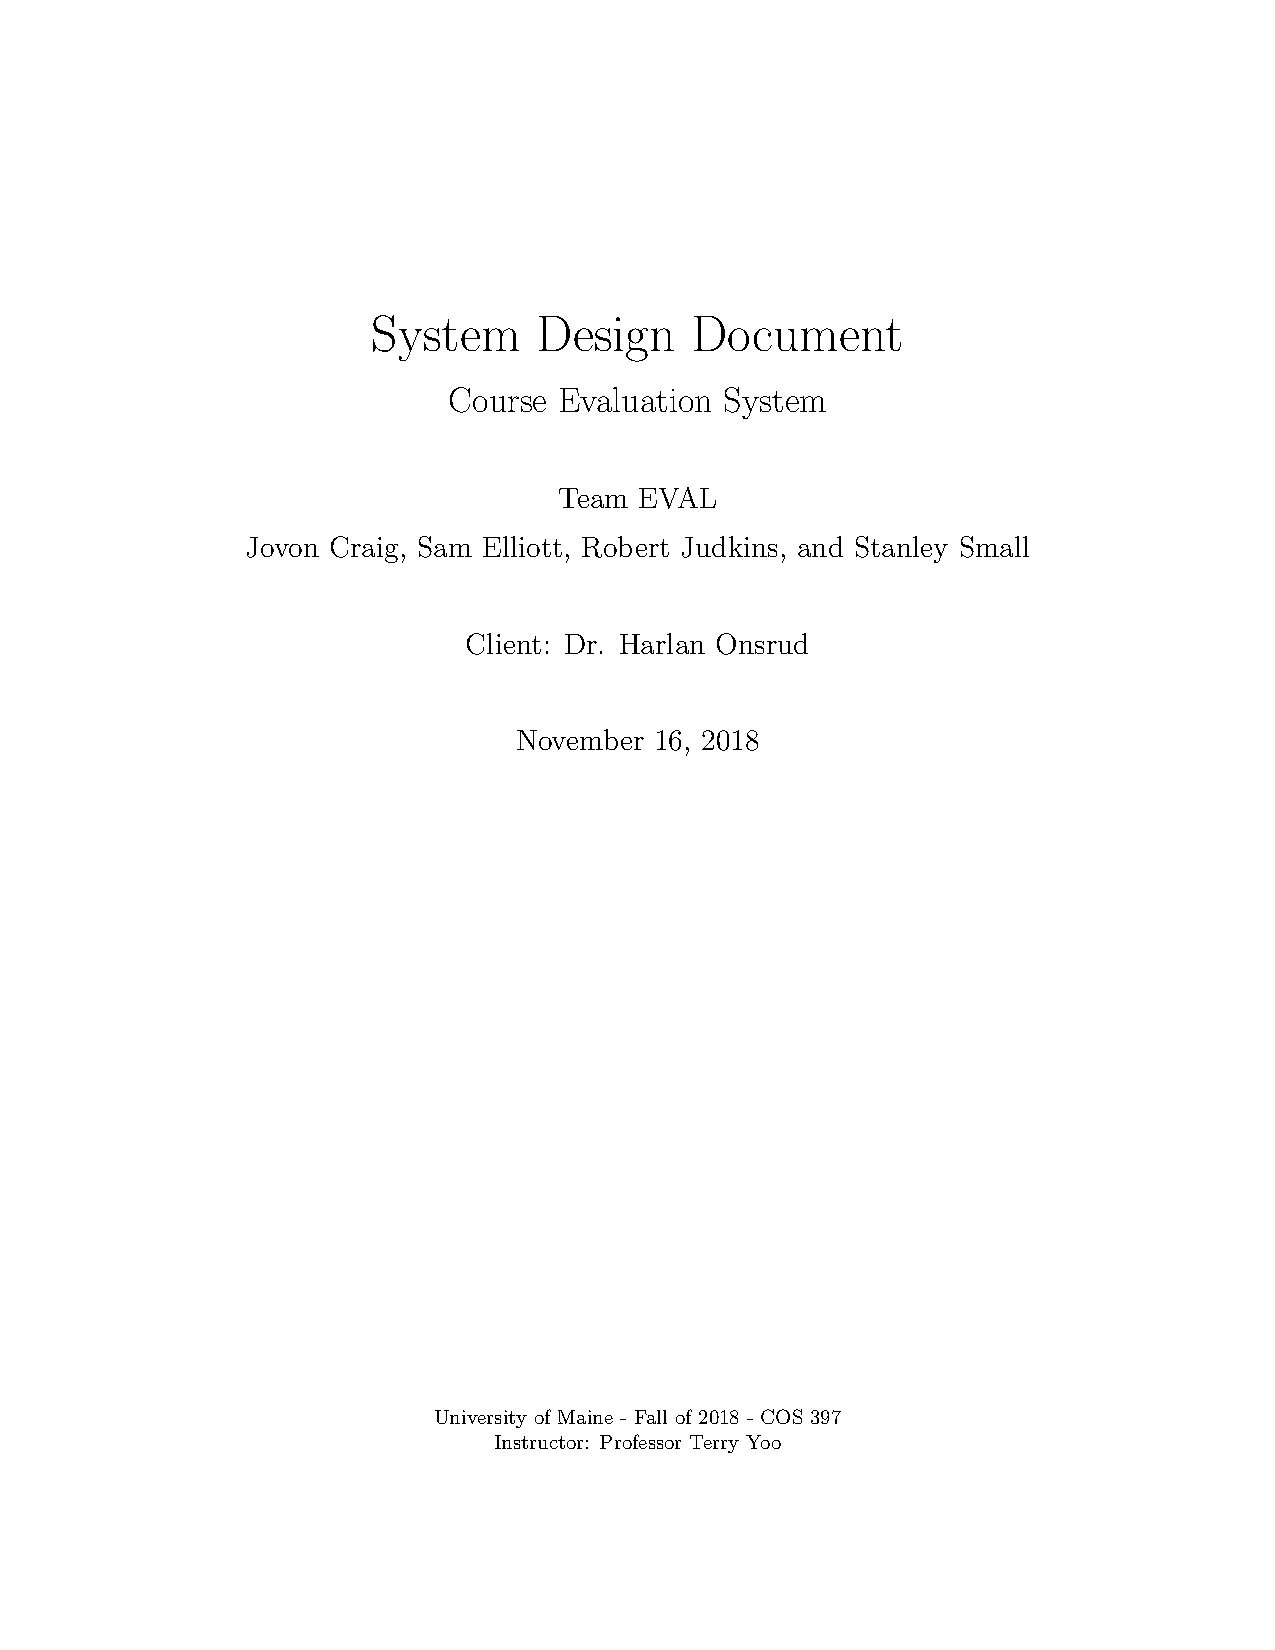
\includepdf[scale=0.85,pages=1,pagecommand=\section{System Design Document}]{sdd.pdf}
\includepdf[scale=0.85,pages=2-]{sdd.pdf}

\newpage

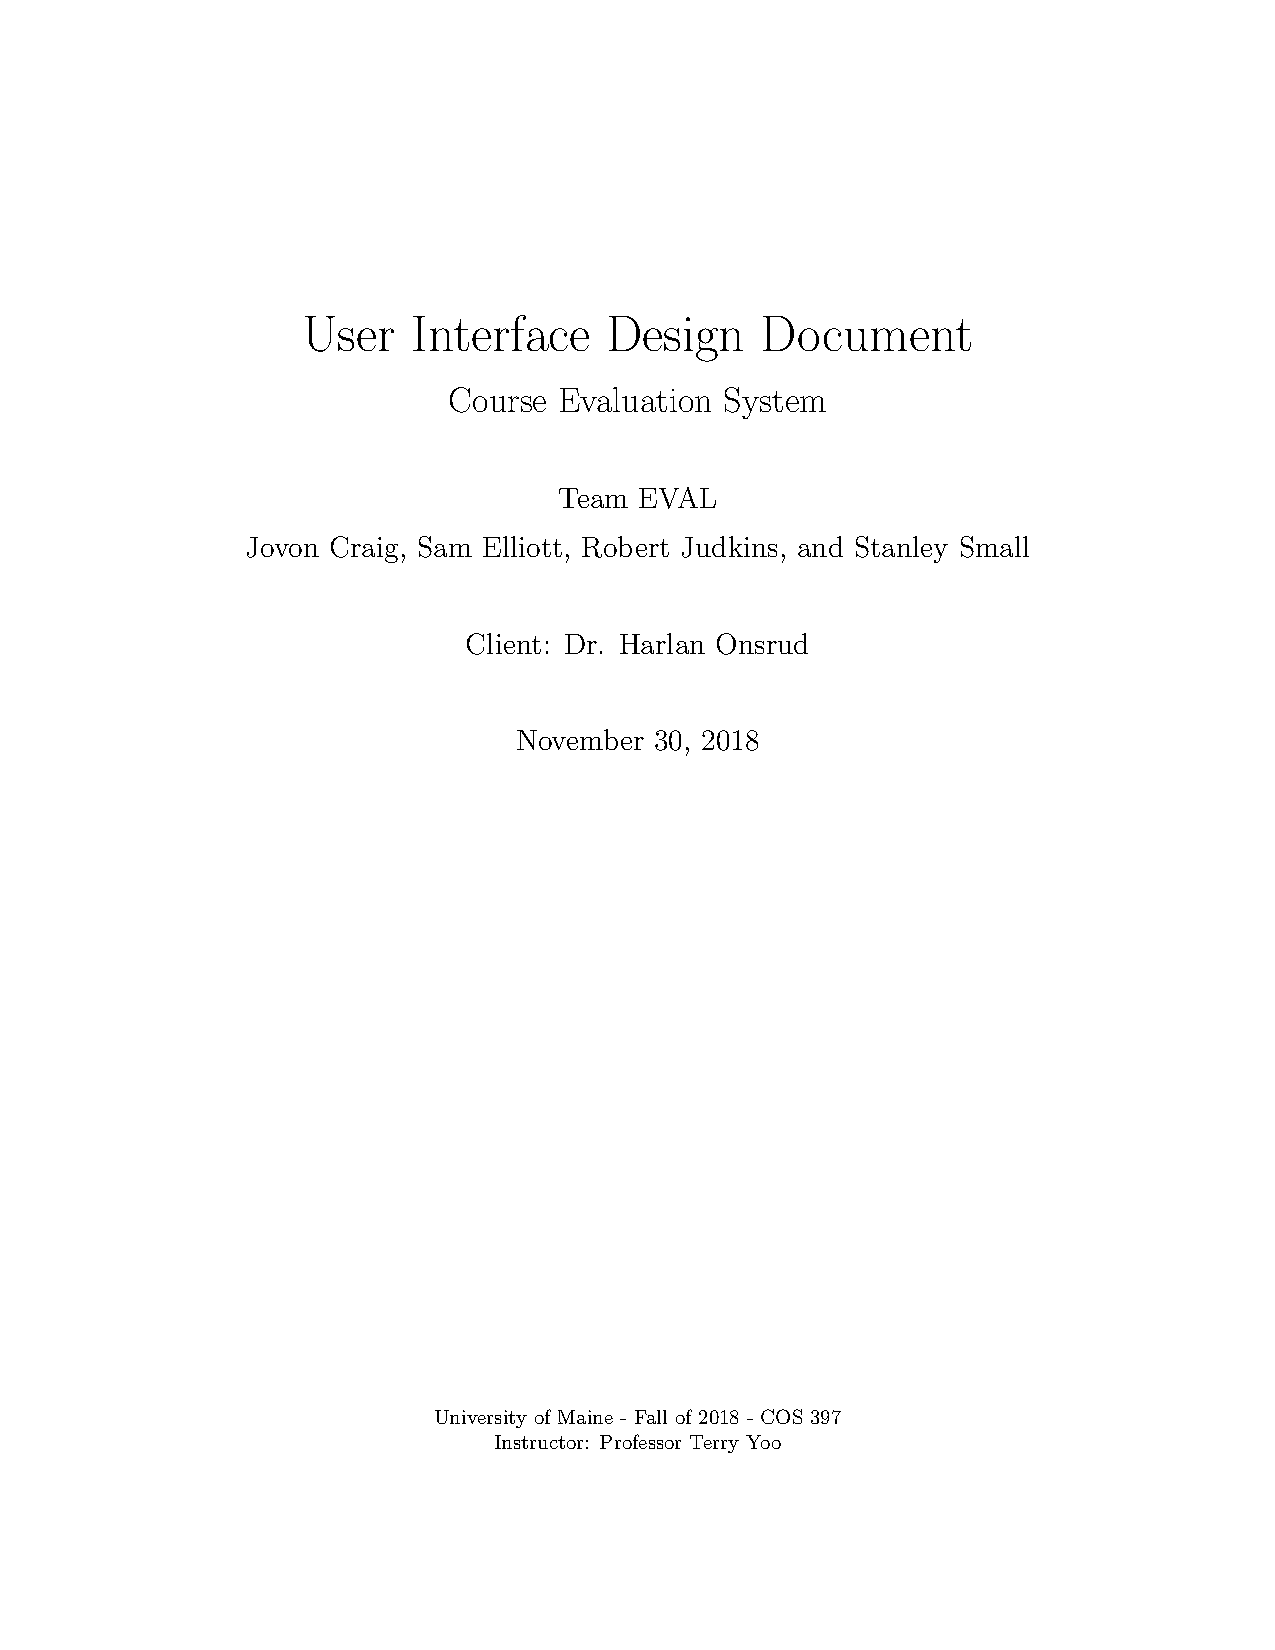
\includepdf[scale=0.85,pages=1,pagecommand=\section{User Interface Design Document}]{uidd.pdf}
\includepdf[scale=0.85,pages=2-]{uidd.pdf}

\newpage

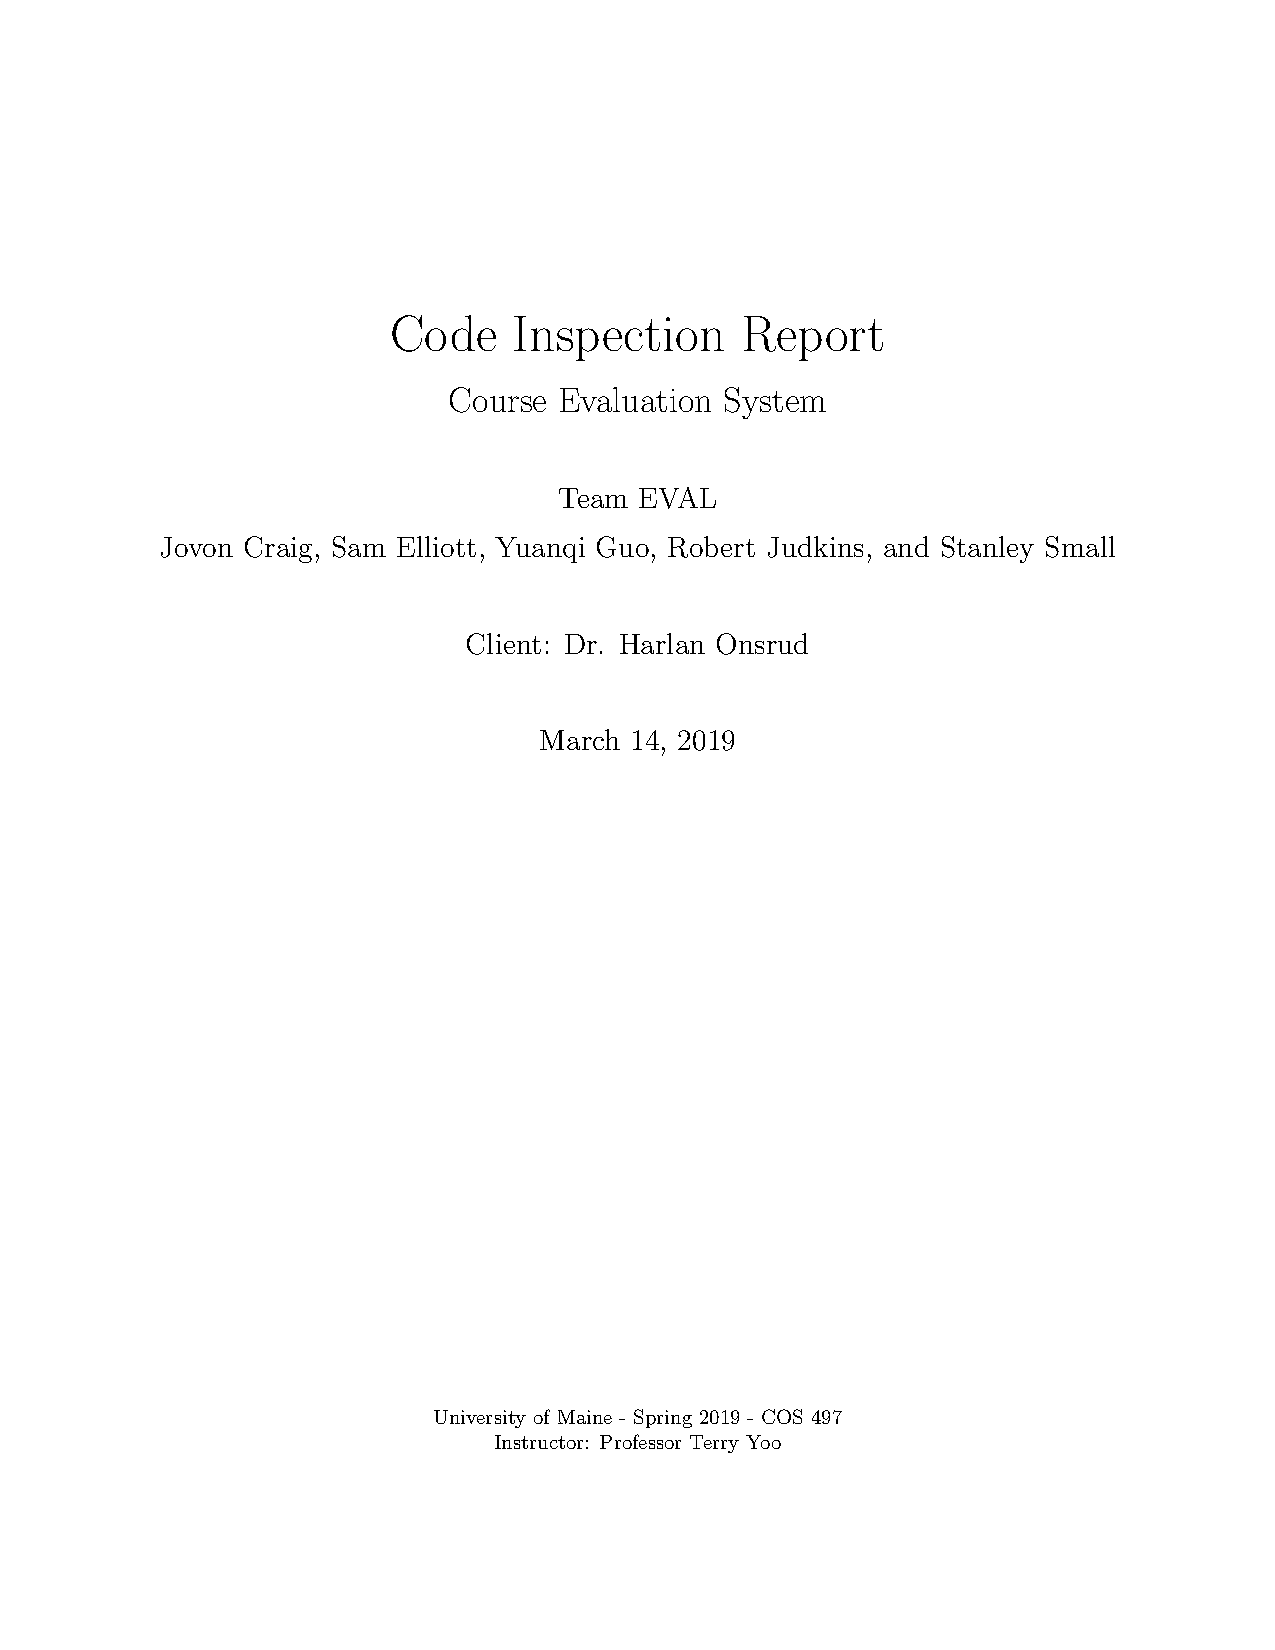
\includepdf[scale=0.85,pages=1,pagecommand=\section{Code Inspection Report}]{cir.pdf}
\includepdf[scale=0.85,pages=2-]{cir.pdf}

\newpage

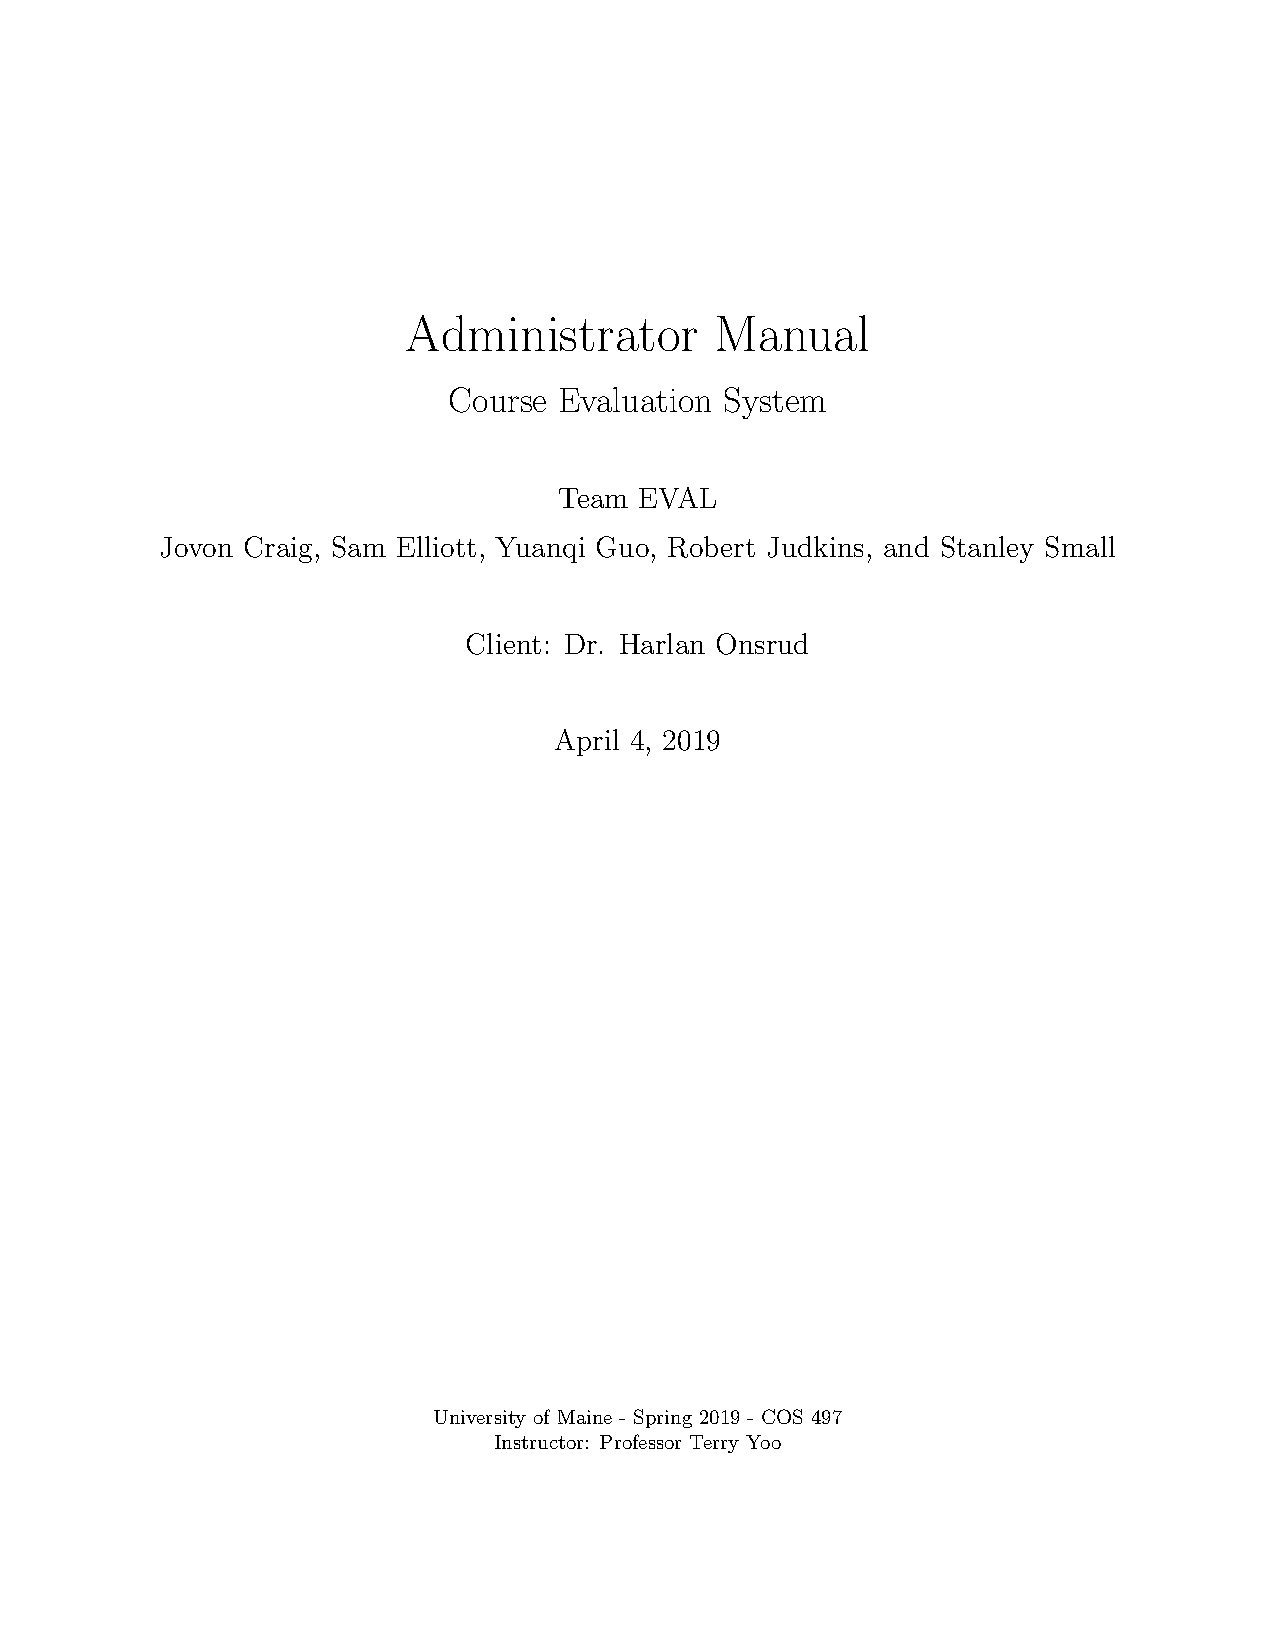
\includepdf[scale=0.85,pages=1,pagecommand=\section{Administrator Manual}]{am.pdf}
\includepdf[scale=0.85,pages=2-]{am.pdf}

\newpage

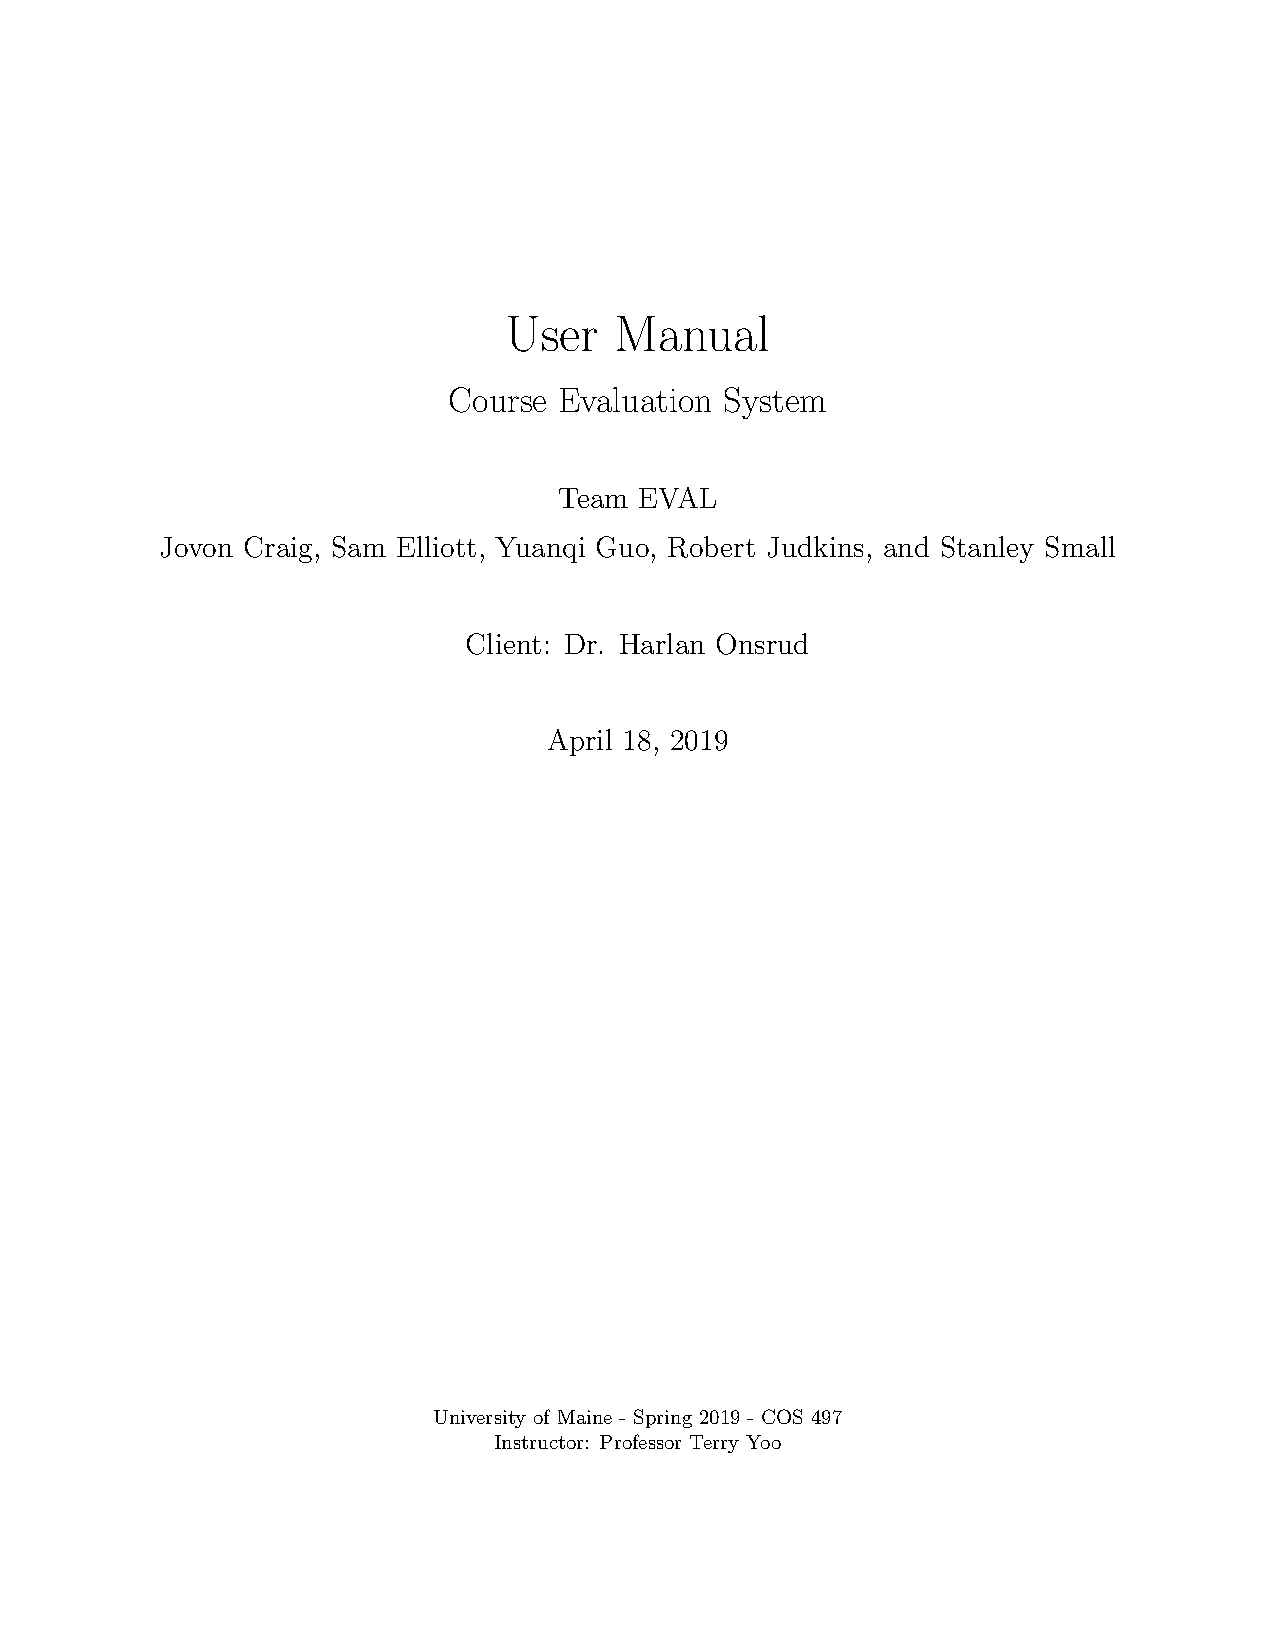
\includepdf[scale=0.85,pages=1,pagecommand=\section{User Manual}]{um.pdf}
\includepdf[scale=0.85,pages=2-]{um.pdf}

\newpage

\includepdf[scale=0.85,pages=1,pagecommand=\section{Example Question Selection Form}]{images/question_appendix.pdf}
\includepdf[scale=0.85,pages=2-]{images/question_appendix.pdf}

\newpage

\includepdf[scale=0.92,pages=1,pagecommand=\section{Example Results Display}]{images/results_appendix.pdf}
\includepdf[scale=0.92,pages=2-]{images/results_appendix.pdf}
\end{document}
